\documentclass[tikz,border=8pt]{standalone}
\usepackage{ctex}
\usepackage{amsmath,amssymb}
\usetikzlibrary{arrows.meta,calc,angles,quotes,patterns,positioning,decorations.pathmorphing}
\definecolor{ink}{RGB}{30,43,58}
\definecolor{blue}{RGB}{38,92,168}
\definecolor{orange}{RGB}{220,112,24}
\definecolor{green}{RGB}{38,139,93}
\definecolor{red}{RGB}{192,53,53}
\tikzset{
 line cap=round,line join=round,
 body/.style={draw=ink,very thick},
 axis/.style={-{Latex[length=2.5mm]},draw=ink,very thick},
 vec/.style={-{Latex[length=2.5mm]},draw=blue,very thick},
 force/.style={-{Latex[length=2.5mm]},draw=red,very thick},
 ray/.style={-{Latex[length=2.2mm]},draw=orange,very thick},
 guide/.style={draw=ink!48,dashed},
 dim/.style={{Latex[length=2mm]}-{Latex[length=2mm]},draw=ink!70}
}

\usetikzlibrary{decorations.pathmorphing}
\tikzset{mass/.style={circle,draw,fill=white,minimum size=7mm},curve/.style={very thick,blue},rope/.style={very thick,blue},ray/.style={very thick,blue,-{Latex}},impulse/.style={very thick,orange,-{Latex}},current/.style={very thick,orange,-{Latex}},resistor/.style={thick,decorate,decoration={zigzag,segment length=3mm,amplitude=1mm}}}
\begin{document}
% 1 question-01
\begin{tikzpicture}[scale=1]
 \coordinate (C) at (0,0);
 \draw[guide] (C) circle(2.8);
 \fill[orange] (-.02,0) circle(8pt) node[above=8pt] {太阳 $M_S$};
 \fill[blue] (2.8,0) circle(4pt) node[right] {地球 $M_E$};
 \fill[red] (0,0) circle(2pt) node[below left] {质心};
 \draw[dim] (0,.35)--(2.8,.35) node[midway,above] {$r_E$};
 \draw[ray] (2.15,.85) arc[start angle=17,end angle=70,radius=1.1];
 \node[blue] at (2.05,1.55) {$\omega$};
 \node[align=center] at (0,-3.45) {恒星光谱的周期性红移与蓝移\\对应太阳的往返径向速度};
\end{tikzpicture}

% 2 solution-01
\begin{tikzpicture}[scale=1]
 \draw[body] (-3.2,0)--(3.2,0);
 % The Sun--barycentre separation is magnified so that both points remain legible.
 \fill[orange] (-.42,0) circle(8pt) node[below left=5pt] {$M_S$};
 \fill[blue] (3.0,0) circle(4pt) node[above right=12pt] {$M_E$};
 \fill[red] (0,0) circle(2pt) node[below right=2pt] {$C$};
 \draw[dim] (-.42,-.65)--(3,-.65) node[midway,below] {$L$};
 \draw[dim] (-.42,.55)--(0,.55) node[midway,above] {$r_S$};
 \draw[dim] (0,.55)--(3,.55) node[midway,above] {$r_E$};
 \node[ink!65] at (-2.25,.75) {间距放大示意};
 \node[align=center] at (0,-1.65)
 {$M_Sr_S=M_Er_E$\quad$r_S+r_E=L$\\[3pt]
  $v_S=\omega L\dfrac{M_E}{M_S+M_E}$};
\end{tikzpicture}

% 3 question-02
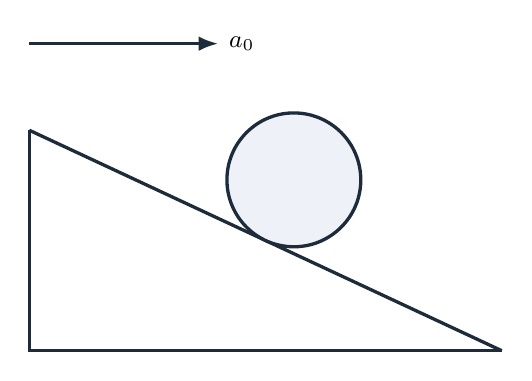
\begin{tikzpicture}[x=1cm,y=1cm,font=\small]
\draw[body] (-3,1.5)--(3,-1.3);\draw[body] (-3,1.5)--(-3,-1.3)--(3,-1.3);\draw[body,fill=blue!8] (0.35945264553145523,0.8702556689959756) circle(.85);\draw[axis] (-3,2.6)--(-.6,2.6) node[right] {$a_0$};
\end{tikzpicture}

% 4 solution-02
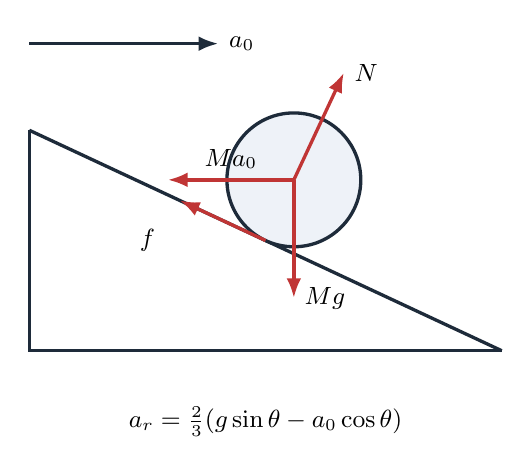
\begin{tikzpicture}[x=1cm,y=1cm,font=\small]
\draw[body] (-3,1.5)--(3,-1.3);\draw[body] (-3,1.5)--(-3,-1.3)--(3,-1.3);\draw[body,fill=blue!8] (0.35945264553145523,0.8702556689959756) circle(.85);\draw[axis] (-3,2.6)--(-.6,2.6) node[right] {$a_0$};\draw[force] (0.35945264553145523,0.8702556689959756)--++(0,-1.5) node[right] {$ Mg $};\draw[force] (0.35945264553145523,0.8702556689959756)--++(-1.6,0) node[midway,above] {$ Ma_0 $};\draw[force] (0.35945264553145523,0.8702556689959756)--++(0.6343281979966857,1.3592747099928981) node[right] {$ N $};\draw[force] plot coordinates {(0.000000,0.100000) (-1.087420,0.607463)};
\node at (-1.5,.1) {$f$};\node at (0,-2.2) {$a_r=\frac23(g\sin\theta-a_0\cos\theta)$};
\end{tikzpicture}

% 5 question-03
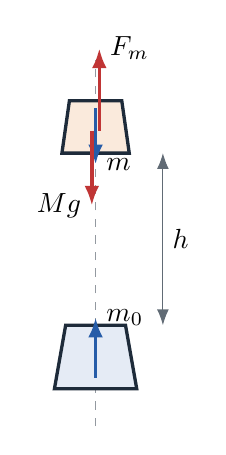
\begin{tikzpicture}[scale=.95]
 \draw[guide] (0,-2.4)--(0,2.5);
 \draw[body,fill=blue!12] (-.55,-1.9)--(.55,-1.9)--(.4,-1.05)--(-.4,-1.05)--cycle;
 \draw[vec] (0,-1.75)--(0,-.95) node[right] {$m_0$};
 \draw[body,fill=orange!15] (-.45,1.25)--(.45,1.25)--(.35,1.95)--(-.35,1.95)--cycle;
 \draw[vec] (0,1.85)--(0,1.1) node[right] {$m$};
 \draw[dim] (.9,-1.05)--(.9,1.25) node[midway,right] {$h$};
 \draw[force] (.05,1.55)--(.05,2.65) node[right] {$F_m$};
 \draw[force] (-.05,1.55)--(-.05,.55) node[left] {$Mg$};
\end{tikzpicture}

% 6 solution-03
\begin{tikzpicture}[scale=.82]
 \begin{scope}[xshift=-5.7cm]
  \draw[axis] (0,0)--(3.8,0) node[below left] {$h+x$};
  \draw[axis] (0,0)--(0,3.0) node[above] {$F$};
  \draw[blue,very thick] plot[smooth] coordinates {(.4,2.8) (.8,1.9) (1.4,1.15) (2.2,.62) (3.3,.3)};
  \draw[red,very thick] (0,1.0)--(3.5,1.0) node[right] {$Mg$};
  \draw[guide] (1.62,0)--(1.62,1.0);
  \fill[ink] (1.62,1.0) circle(2pt) node[below right] {$h$};
  \node at (1.8,-1.3) {$F_m\propto(h+x)^{-4}$};
 \end{scope}
 \begin{scope}[xshift=.1cm]
  \draw[guide] (0,-2)--(0,2.2);
  \draw[body,fill=orange!12] (0,0) ellipse(.75 and .35);
  \draw[vec] (0,0)--(.75,1.85) node[right] {$\boldsymbol L$};
  \draw[force] (.75,1.85)--(-.2,2.25) node[left] {$\boldsymbol\tau$};
  \draw[blue,very thick,-{Latex}] (.75,1.85) arc[start angle=0,end angle=120,x radius=.75,y radius=.22];
  \node at (1.15,1.25) {$\Omega$};

 \end{scope}
 \begin{scope}[xshift=4.4cm]
  \draw[axis] (0,-2.1)--(0,2.2) node[above] {竖直};
  \draw[blue,very thick] plot[domain=-1.8:1.8,samples=80] (\x,{.38*cos(400*\x)+.42*\x});
  \draw[guide] (-1.8,-.8)--(1.8,.8);
  \node[align=center,font=\small] at (0,-2.65)
  {高频快振动叠加慢角运动\\
   $B_c=\omega\sqrt{2I_0B_0/m}$；$B_1>B_c$};
 \end{scope}
\node at (0,-4.05) {$\displaystyle\Omega_\pm=\frac{\omega_0\pm\sqrt{\omega_0^2-4mB_0/I_0}}2$};
\end{tikzpicture}

% 7 question-04
\begin{tikzpicture}[x=1cm,y=1cm,font=\small]
\begin{scope}[xshift=-3.8cm]\coordinate(C) at(0,2.4);\draw[rope] (C)--(0,.9) (C)--(0,-1.5);\draw[body,line width=2pt] (0,.9)--(0,-1.5);\node[left] at(0,.9){$B,m_2$};\node[left] at(0,-1.5){$A,m_1$};\node at(0,-2.2){I：$\delta<c/a$ 稳定};\end{scope}\begin{scope}[xshift=.1cm]\coordinate(C) at(0,2.4);\draw[rope] (C)--(0,.9) (C)--(0,-1.5);\draw[body,line width=2pt] (0,.9)--(0,-1.5);\node[left] at(0,.9){$A,m_1$};\node[left] at(0,-1.5){$B,m_2$};\node at(0,-2.2){II：稳定};\end{scope}\begin{scope}[xshift=4.2cm,yshift=2.4cm]\draw[rope] plot coordinates {(0.000000,0.000000) (-1.309898,-2.619052) (1.180753,-2.360836) (0.000000,0.000000)};
\draw[body,line width=2pt] plot coordinates {(-1.309898,-2.619052) (1.180753,-2.360836)};
\fill (-1.309898,-2.619052) circle(2pt) node[below] {$A$};
\fill (1.180753,-2.360836) circle(2pt) node[below] {$B$};
\fill (0.000000,-2.483249) circle(2pt) node[below] {$H$};
\draw[guide] (0,0)--(0,-3);\node[above] at(0,0){$C$};\node at(0,-4.6){III：鞍点};\end{scope}
\end{tikzpicture}

% 8 solution-04
\begin{tikzpicture}[x=1cm,y=1cm,font=\small]
\begin{scope}[xshift=-3.8cm]\coordinate(C) at(0,2.4);\draw[rope] (C)--(0,.9) (C)--(0,-1.5);\draw[body,line width=2pt] (0,.9)--(0,-1.5);\node[left] at(0,.9){$B,m_2$};\node[left] at(0,-1.5){$A,m_1$};\node at(0,-2.2){I：$\delta<c/a$ 稳定};\end{scope}\begin{scope}[xshift=.1cm]\coordinate(C) at(0,2.4);\draw[rope] (C)--(0,.9) (C)--(0,-1.5);\draw[body,line width=2pt] (0,.9)--(0,-1.5);\node[left] at(0,.9){$A,m_1$};\node[left] at(0,-1.5){$B,m_2$};\node at(0,-2.2){II：稳定};\end{scope}\begin{scope}[xshift=4.2cm,yshift=2.4cm]\draw[rope] plot coordinates {(0.000000,0.000000) (-1.309898,-2.619052) (1.180753,-2.360836) (0.000000,0.000000)};
\draw[body,line width=2pt] plot coordinates {(-1.309898,-2.619052) (1.180753,-2.360836)};
\fill (-1.309898,-2.619052) circle(2pt) node[below] {$A$};
\fill (1.180753,-2.360836) circle(2pt) node[below] {$B$};
\fill (0.000000,-2.483249) circle(2pt) node[below] {$H$};
\draw[guide] (0,0)--(0,-3);\node[above] at(0,0){$C$};\node at(0,-4.6){III：鞍点};\end{scope}\node at(0,-3.2){$\det K_I\propto M-a(m_2-m_1)/c$；二自由度判定稳定性};
\end{tikzpicture}

% 9 question-05
\begin{tikzpicture}[scale=1]
 \fill[ink!8] (-3,-2.0) rectangle (-2.75,2.3);
 \draw[body,line width=3pt] (-2.75,-2.0)--(-2.75,2.3);
 \draw[body,fill=blue!10] (.5,0) circle(1.1);
 \fill[ink] (.5,0) circle(2pt);
 \draw[dim] (-2.75,.25)--(.5,.25) node[midway,above] {$l$};
 \draw[dim] (.5,0)--(1.6,0) node[midway,below] {$r$};
 \node[rotate=90] at (-3.25,0) {接地导体平面};
 \node at (.5,-1.55) {无限长圆柱截面};
\end{tikzpicture}

% 10 solution-05
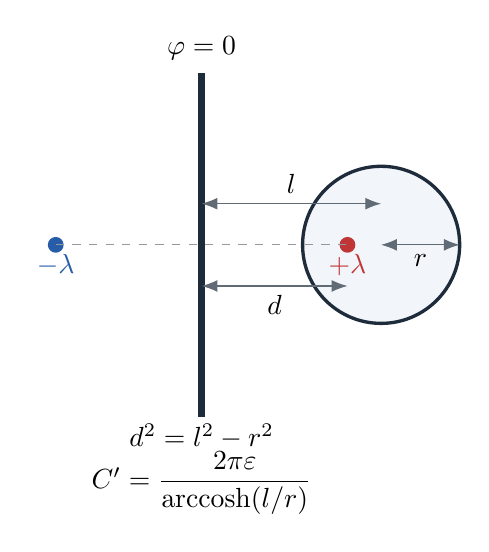
\begin{tikzpicture}[scale=.95]
 \draw[body,line width=2.5pt] (0,-2.3)--(0,2.3) node[above] {$\varphi=0$};
 \draw[body,fill=blue!6] (2.4,0) circle(1.05);
 \fill[red] (1.95,0) circle(3pt) node[below] {$+\lambda$};
 \fill[blue] (-1.95,0) circle(3pt) node[below] {$-\lambda$};
 \draw[guide] (-1.95,0)--(1.95,0);
 \draw[dim] (0,.55)--(2.4,.55) node[midway,above] {$l$};
 \draw[dim] (1.95,-.55)--(0,-.55) node[midway,below] {$d$};
 \draw[dim] (2.4,0)--(3.45,0) node[midway,below] {$r$};
 \node[align=center] at (0,-3.0)
 {$d^2=l^2-r^2$\\
  $C'=\dfrac{2\pi\varepsilon}{\operatorname{arccosh}(l/r)}$};
\end{tikzpicture}

% 11 question-06
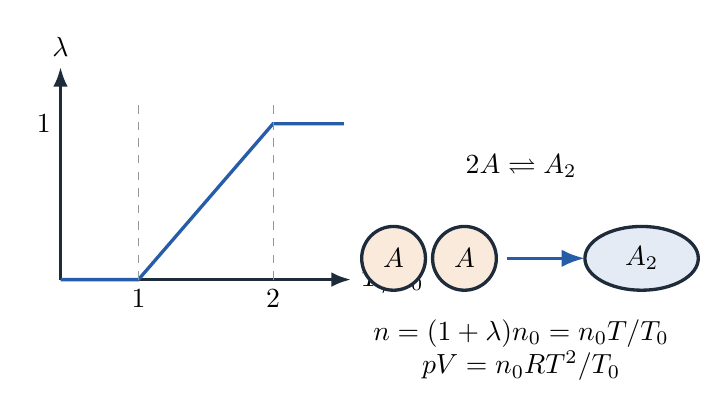
\begin{tikzpicture}[scale=.9]
 \begin{scope}[xshift=-3.8cm]
  \draw[axis] (0,0)--(4.1,0) node[right] {$T/T_0$};
  \draw[axis] (0,0)--(0,3.0) node[above] {$\lambda$};
  \draw[blue,very thick] (0,0)--(1.1,0)--(3.0,2.2)--(4.0,2.2);
  \draw[guide] (1.1,0)--(1.1,2.5); \draw[guide] (3,0)--(3,2.5);
  \node[below] at (1.1,0) {$1$}; \node[below] at (3,0) {$2$};
  \node[left] at (0,2.2) {$1$};
 \end{scope}
 \begin{scope}[xshift=2.7cm]
  \node at (0,1.6) {$2A\rightleftharpoons A_2$};
  \draw[body,fill=orange!15] (-1.8,.3) circle(.45) node {$A$};
  \draw[body,fill=orange!15] (-.8,.3) circle(.45) node {$A$};
  \draw[blue,very thick,-{Latex}] (-.2,.3)--(.9,.3);
  \draw[body,fill=blue!12] (1.7,.3) ellipse(.8 and .45) node {$A_2$};
  \node[align=center] at (0,-1.0)
  {$n=(1+\lambda)n_0=n_0T/T_0$\\$pV=n_0RT^2/T_0$};
 \end{scope}
\end{tikzpicture}

% 12 solution-06
\begin{tikzpicture}[scale=.92]
 \draw[axis] (0,0)--(5.7,0) node[right] {$V$};
 \draw[axis] (0,0)--(0,4.0) node[above] {$p$};
 % Volumes differ by powers of 2^6; the horizontal spacings are schematic.
 \coordinate (A) at (2.75,1.35); \coordinate (B) at (4.85,.72);
 \coordinate (C) at (1.45,3.02); \coordinate (D) at (.72,3.55);
 \draw[blue,very thick,-{Latex}] (A) to[out=-15,in=180] (B);
 \draw[orange,very thick,-{Latex}] (B) to[out=150,in=-35] (C);
 \draw[red,very thick,-{Latex}] (C) to[out=155,in=-10] (D);
 \draw[green,very thick,-{Latex}] (D) to[out=-75,in=150] (A);
 \foreach \p/\lab/\pos in {A/A/left,B/B/below,C/C/right,D/D/above}{\fill[ink] (\p) circle(2.5pt) node[\pos] {$\lab$};}
 \node[blue] at (3.95,.28) {$T_0$ 等温膨胀};
 \node[red] at (2.75,3.46) {$2T_0$ 等温压缩};
 \node[orange,fill=white,inner sep=1pt,rotate=31] at (3.15,2.15) {形式绝热压缩};
 \node[green!80!black,fill=white,inner sep=1pt,rotate=-38] at (1.55,1.86) {形式绝热膨胀};
 \node[ink!65] at (1.65,-.48) {体积轴为示意比例};
 \node[draw=ink!35,rounded corners,fill=white,align=left,inner sep=5pt] at (6.65,2.0)
 {$A\to B:\ Q_1=n_0RT_0\ln2$\\[2pt]
  $C\to D:\ Q_2=4n_0RT_0\ln2$};
\end{tikzpicture}

% 13 question-07
\begin{tikzpicture}[scale=.78]
 \begin{scope}[xshift=-5.3cm]
  \draw[body] (-2,0) .. controls (-.8,.65) and (.8,-.65) .. (2,0);
  \draw[force] (-1.5,.25)--(-2.25,.75) node[left] {$2\sigma$};
  \draw[force] (1.5,-.25)--(2.25,-.75) node[right] {$2\sigma$};
  \node at (0,-1.2) {横波膜元};
 \end{scope}
 \begin{scope}
  \draw[body] (0,0) ellipse(2.0 and .65);
  \draw[blue,very thick] (-2,0) .. controls (-1.0,-1.15) and (1.0,-1.15) .. (2,0);
  \draw[dim] (0,0)--(2,0) node[midway,above] {$r$};
  \draw[dim] (0,0)--(0,-.8) node[midway,right] {$h_0$};
  \node at (0,-1.7) {水平圆膜重力下沉};
 \end{scope}
 \begin{scope}[xshift=5.0cm]
  \draw[body] (0,1.5) ellipse(1.15 and .38);
  \draw[body] (0,-1.3) ellipse(2.0 and .65);
  \draw[blue,very thick] (-1.15,1.5) .. controls (-1.55,.45) and (-2,-.2) .. (-2,-1.3);
  \draw[blue,very thick] (1.15,1.5) .. controls (1.55,.45) and (2,-.2) .. (2,-1.3);
  \draw[dim] (2.5,-1.3)--(2.5,1.5) node[midway,right] {$h_0$};
  \node at (0,-2.25) {同轴双圆环};
 \end{scope}
\end{tikzpicture}

% 14 solution-07
\begin{tikzpicture}[scale=.8]
 \begin{scope}[xshift=-5.1cm]
  \draw[axis] (-2.2,0)--(2.4,0) node[right] {$x$};
  \draw[axis] (0,-.2)--(0,2.5) node[above] {$h$};
  \draw[blue,very thick] plot[domain=-2:2,samples=80] (\x,{1.7-.42*\x*\x});
  \draw[guide] (-2,0)--(-2,1.7); \draw[guide] (2,0)--(2,1.7);
  \node at (0,-.75) {$h(x)=\dfrac{\rho g}{8\sigma}(r^2-x^2)$};
 \end{scope}
 \begin{scope}
  \draw[axis] (0,0)--(4.4,0) node[right] {$x$};
  \draw[axis] (0,0)--(0,3.0) node[above] {$z$};
  \draw[blue,very thick] plot[smooth] coordinates {(.6,2.4) (1.0,2.0) (1.8,1.35) (2.8,.7) (3.8,0)};
  \draw[guide] (.6,0)--(.6,2.4); \draw[guide] (3.8,0)--(3.8,0);
  \node[below] at (.6,0) {$r_2$}; \node[below] at (3.8,0) {$r_1$};
  \node at (2.2,-.85) {$z''+z'/x=\rho g/(2\sigma)$};
 \end{scope}
 \begin{scope}[xshift=5.0cm]
  \draw[body] (-2,0)--(2,0);
  \draw[blue,very thick] (-2,0) .. controls (-1,-1.1) and (1,-1.1) .. (2,0);
  \draw[force] (0,-.8)--(0,-1.8) node[below] {$\pi x^2\rho g$};
  \draw[force] (-1.4,-.45)--(-1.8,.45) node[left] {$2\sigma$};
  \draw[force] (1.4,-.45)--(1.8,.45) node[right] {$2\sigma$};
  \node at (0,1.1) {圆周张力支撑膜重};
 \end{scope}
\end{tikzpicture}

% 15 question-08
\begin{tikzpicture}[scale=.9]
 \begin{scope}[xshift=-3.7cm]
  \draw[body,fill=blue!8] (0,-1.6) rectangle (3.0,1.6);
  \draw[ray] (-3,0)--(0,0)--(2.7,0);
  \draw[vec] (2.5,1.05)--(.65,1.05) node[midway,above] {$\beta c$};
  \node at (1.5,-1.95) {运动介质 $n$};
  \foreach \x in {-2.7,-2.2,-1.7,-1.2,-.7}{\draw[orange] (\x,-.45)--(\x,.45);}
  \foreach \x in {.35,.85,1.35,1.85,2.35}{\draw[blue] (\x,-.45)--(\x,.45);}
 \end{scope}
 \begin{scope}[xshift=3.2cm]
  \draw[axis] (-.2,0)--(4.8,0) node[right] {$x$};
  \draw[axis] (0,-2.2)--(0,2.2) node[above] {$\rho$};
  \foreach \y in {-1.6,-.8,.8,1.6}{
   \draw[vec] (.2,\y)--({.7+0.42*\y*\y},\y);}
  \draw[orange,very thick] (0,-1.8)--(0,1.8);
  \draw[blue,very thick] (4,0) .. controls (2.5,.65) and (1.5,1.2) .. (0,1.6);
  \draw[blue,very thick] (4,0) .. controls (2.5,-.65) and (1.5,-1.2) .. (0,-1.6);
  \fill[red] (4,0) circle(3pt) node[above] {焦点};
  \node at (2.2,-2.65) {$u(\rho)=c\rho^2/\rho_0^2$};
 \end{scope}
\end{tikzpicture}

% 16 solution-08
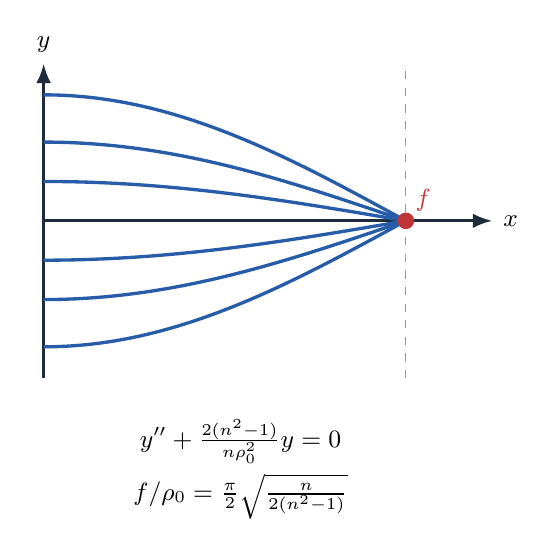
\begin{tikzpicture}[x=1cm,y=1cm,font=\small]
\draw[axis] (0,0)--(5.7,0) node[right] {$x$};\draw[axis] (0,-2)--(0,2) node[above] {$y$};\draw[blue,very thick] plot coordinates {(0.000000,-1.600000) (0.051685,-1.599751) (0.103371,-1.599003) (0.155056,-1.597758) (0.206742,-1.596014) (0.258427,-1.593774) (0.310112,-1.591037) (0.361798,-1.587805) (0.413483,-1.584078) (0.465169,-1.579857) (0.516854,-1.575145) (0.568539,-1.569941) (0.620225,-1.564249) (0.671910,-1.558069) (0.723596,-1.551405) (0.775281,-1.544257) (0.826966,-1.536627) (0.878652,-1.528520) (0.930337,-1.519936) (0.982022,-1.510878) (1.033708,-1.501350) (1.085393,-1.491355) (1.137079,-1.480895) (1.188764,-1.469973) (1.240449,-1.458594) (1.292135,-1.446760) (1.343820,-1.434476) (1.395506,-1.421744) (1.447191,-1.408570) (1.498876,-1.394958) (1.550562,-1.380910) (1.602247,-1.366433) (1.653933,-1.351530) (1.705618,-1.336205) (1.757303,-1.320465) (1.808989,-1.304314) (1.860674,-1.287756) (1.912360,-1.270797) (1.964045,-1.253442) (2.015730,-1.235696) (2.067416,-1.217566) (2.119101,-1.199057) (2.170787,-1.180174) (2.222472,-1.160923) (2.274157,-1.141311) (2.325843,-1.121343) (2.377528,-1.101026) (2.429213,-1.080366) (2.480899,-1.059369) (2.532584,-1.038043) (2.584270,-1.016393) (2.635955,-0.994426) (2.687640,-0.972150) (2.739326,-0.949571) (2.791011,-0.926696) (2.842697,-0.903533) (2.894382,-0.880088) (2.946067,-0.856369) (2.997753,-0.832383) (3.049438,-0.808138) (3.101124,-0.783641) (3.152809,-0.758900) (3.204494,-0.733923) (3.256180,-0.708717) (3.307865,-0.683290) (3.359551,-0.657651) (3.411236,-0.631806) (3.462921,-0.605765) (3.514607,-0.579535) (3.566292,-0.553125) (3.617978,-0.526542) (3.669663,-0.499795) (3.721348,-0.472893) (3.773034,-0.445843) (3.824719,-0.418655) (3.876404,-0.391336) (3.928090,-0.363895) (3.979775,-0.336341) (4.031461,-0.308682) (4.083146,-0.280927) (4.134831,-0.253084) (4.186517,-0.225162) (4.238202,-0.197171) (4.289888,-0.169118) (4.341573,-0.141012) (4.393258,-0.112862) (4.444944,-0.084678) (4.496629,-0.056466) (4.548315,-0.028238) (4.600000,-0.000000)};
\draw[blue,very thick] plot coordinates {(0.000000,-1.000000) (0.051685,-0.999844) (0.103371,-0.999377) (0.155056,-0.998599) (0.206742,-0.997509) (0.258427,-0.996109) (0.310112,-0.994398) (0.361798,-0.992378) (0.413483,-0.990049) (0.465169,-0.987411) (0.516854,-0.984465) (0.568539,-0.981213) (0.620225,-0.977656) (0.671910,-0.973793) (0.723596,-0.969628) (0.775281,-0.965160) (0.826966,-0.960392) (0.878652,-0.955325) (0.930337,-0.949960) (0.982022,-0.944299) (1.033708,-0.938344) (1.085393,-0.932097) (1.137079,-0.925559) (1.188764,-0.918733) (1.240449,-0.911621) (1.292135,-0.904225) (1.343820,-0.896547) (1.395506,-0.888590) (1.447191,-0.880356) (1.498876,-0.871848) (1.550562,-0.863069) (1.602247,-0.854020) (1.653933,-0.844706) (1.705618,-0.835128) (1.757303,-0.825291) (1.808989,-0.815196) (1.860674,-0.804847) (1.912360,-0.794248) (1.964045,-0.783401) (2.015730,-0.772310) (2.067416,-0.760979) (2.119101,-0.749410) (2.170787,-0.737608) (2.222472,-0.725577) (2.274157,-0.713319) (2.325843,-0.700839) (2.377528,-0.688141) (2.429213,-0.675229) (2.480899,-0.662106) (2.532584,-0.648777) (2.584270,-0.635246) (2.635955,-0.621517) (2.687640,-0.607594) (2.739326,-0.593482) (2.791011,-0.579185) (2.842697,-0.564708) (2.894382,-0.550055) (2.946067,-0.535231) (2.997753,-0.520239) (3.049438,-0.505086) (3.101124,-0.489776) (3.152809,-0.474313) (3.204494,-0.458702) (3.256180,-0.442948) (3.307865,-0.427056) (3.359551,-0.411032) (3.411236,-0.394879) (3.462921,-0.378603) (3.514607,-0.362210) (3.566292,-0.345703) (3.617978,-0.329089) (3.669663,-0.312372) (3.721348,-0.295558) (3.773034,-0.278652) (3.824719,-0.261659) (3.876404,-0.244585) (3.928090,-0.227434) (3.979775,-0.210213) (4.031461,-0.192926) (4.083146,-0.175579) (4.134831,-0.158177) (4.186517,-0.140726) (4.238202,-0.123232) (4.289888,-0.105699) (4.341573,-0.088132) (4.393258,-0.070539) (4.444944,-0.052923) (4.496629,-0.035291) (4.548315,-0.017648) (4.600000,-0.000000)};
\draw[blue,very thick] plot coordinates {(0.000000,-0.500000) (0.051685,-0.499922) (0.103371,-0.499689) (0.155056,-0.499299) (0.206742,-0.498755) (0.258427,-0.498054) (0.310112,-0.497199) (0.361798,-0.496189) (0.413483,-0.495024) (0.465169,-0.493705) (0.516854,-0.492233) (0.568539,-0.490607) (0.620225,-0.488828) (0.671910,-0.486897) (0.723596,-0.484814) (0.775281,-0.482580) (0.826966,-0.480196) (0.878652,-0.477662) (0.930337,-0.474980) (0.982022,-0.472149) (1.033708,-0.469172) (1.085393,-0.466048) (1.137079,-0.462780) (1.188764,-0.459367) (1.240449,-0.455811) (1.292135,-0.452112) (1.343820,-0.448274) (1.395506,-0.444295) (1.447191,-0.440178) (1.498876,-0.435924) (1.550562,-0.431534) (1.602247,-0.427010) (1.653933,-0.422353) (1.705618,-0.417564) (1.757303,-0.412645) (1.808989,-0.407598) (1.860674,-0.402424) (1.912360,-0.397124) (1.964045,-0.391701) (2.015730,-0.386155) (2.067416,-0.380489) (2.119101,-0.374705) (2.170787,-0.368804) (2.222472,-0.362788) (2.274157,-0.356660) (2.325843,-0.350420) (2.377528,-0.344071) (2.429213,-0.337614) (2.480899,-0.331053) (2.532584,-0.324388) (2.584270,-0.317623) (2.635955,-0.310758) (2.687640,-0.303797) (2.739326,-0.296741) (2.791011,-0.289593) (2.842697,-0.282354) (2.894382,-0.275028) (2.946067,-0.267615) (2.997753,-0.260120) (3.049438,-0.252543) (3.101124,-0.244888) (3.152809,-0.237156) (3.204494,-0.229351) (3.256180,-0.221474) (3.307865,-0.213528) (3.359551,-0.205516) (3.411236,-0.197439) (3.462921,-0.189302) (3.514607,-0.181105) (3.566292,-0.172852) (3.617978,-0.164544) (3.669663,-0.156186) (3.721348,-0.147779) (3.773034,-0.139326) (3.824719,-0.130830) (3.876404,-0.122292) (3.928090,-0.113717) (3.979775,-0.105106) (4.031461,-0.096463) (4.083146,-0.087790) (4.134831,-0.079089) (4.186517,-0.070363) (4.238202,-0.061616) (4.289888,-0.052849) (4.341573,-0.044066) (4.393258,-0.035269) (4.444944,-0.026462) (4.496629,-0.017646) (4.548315,-0.008824) (4.600000,-0.000000)};
\draw[blue,very thick] plot coordinates {(0.000000,0.500000) (0.051685,0.499922) (0.103371,0.499689) (0.155056,0.499299) (0.206742,0.498755) (0.258427,0.498054) (0.310112,0.497199) (0.361798,0.496189) (0.413483,0.495024) (0.465169,0.493705) (0.516854,0.492233) (0.568539,0.490607) (0.620225,0.488828) (0.671910,0.486897) (0.723596,0.484814) (0.775281,0.482580) (0.826966,0.480196) (0.878652,0.477662) (0.930337,0.474980) (0.982022,0.472149) (1.033708,0.469172) (1.085393,0.466048) (1.137079,0.462780) (1.188764,0.459367) (1.240449,0.455811) (1.292135,0.452112) (1.343820,0.448274) (1.395506,0.444295) (1.447191,0.440178) (1.498876,0.435924) (1.550562,0.431534) (1.602247,0.427010) (1.653933,0.422353) (1.705618,0.417564) (1.757303,0.412645) (1.808989,0.407598) (1.860674,0.402424) (1.912360,0.397124) (1.964045,0.391701) (2.015730,0.386155) (2.067416,0.380489) (2.119101,0.374705) (2.170787,0.368804) (2.222472,0.362788) (2.274157,0.356660) (2.325843,0.350420) (2.377528,0.344071) (2.429213,0.337614) (2.480899,0.331053) (2.532584,0.324388) (2.584270,0.317623) (2.635955,0.310758) (2.687640,0.303797) (2.739326,0.296741) (2.791011,0.289593) (2.842697,0.282354) (2.894382,0.275028) (2.946067,0.267615) (2.997753,0.260120) (3.049438,0.252543) (3.101124,0.244888) (3.152809,0.237156) (3.204494,0.229351) (3.256180,0.221474) (3.307865,0.213528) (3.359551,0.205516) (3.411236,0.197439) (3.462921,0.189302) (3.514607,0.181105) (3.566292,0.172852) (3.617978,0.164544) (3.669663,0.156186) (3.721348,0.147779) (3.773034,0.139326) (3.824719,0.130830) (3.876404,0.122292) (3.928090,0.113717) (3.979775,0.105106) (4.031461,0.096463) (4.083146,0.087790) (4.134831,0.079089) (4.186517,0.070363) (4.238202,0.061616) (4.289888,0.052849) (4.341573,0.044066) (4.393258,0.035269) (4.444944,0.026462) (4.496629,0.017646) (4.548315,0.008824) (4.600000,0.000000)};
\draw[blue,very thick] plot coordinates {(0.000000,1.000000) (0.051685,0.999844) (0.103371,0.999377) (0.155056,0.998599) (0.206742,0.997509) (0.258427,0.996109) (0.310112,0.994398) (0.361798,0.992378) (0.413483,0.990049) (0.465169,0.987411) (0.516854,0.984465) (0.568539,0.981213) (0.620225,0.977656) (0.671910,0.973793) (0.723596,0.969628) (0.775281,0.965160) (0.826966,0.960392) (0.878652,0.955325) (0.930337,0.949960) (0.982022,0.944299) (1.033708,0.938344) (1.085393,0.932097) (1.137079,0.925559) (1.188764,0.918733) (1.240449,0.911621) (1.292135,0.904225) (1.343820,0.896547) (1.395506,0.888590) (1.447191,0.880356) (1.498876,0.871848) (1.550562,0.863069) (1.602247,0.854020) (1.653933,0.844706) (1.705618,0.835128) (1.757303,0.825291) (1.808989,0.815196) (1.860674,0.804847) (1.912360,0.794248) (1.964045,0.783401) (2.015730,0.772310) (2.067416,0.760979) (2.119101,0.749410) (2.170787,0.737608) (2.222472,0.725577) (2.274157,0.713319) (2.325843,0.700839) (2.377528,0.688141) (2.429213,0.675229) (2.480899,0.662106) (2.532584,0.648777) (2.584270,0.635246) (2.635955,0.621517) (2.687640,0.607594) (2.739326,0.593482) (2.791011,0.579185) (2.842697,0.564708) (2.894382,0.550055) (2.946067,0.535231) (2.997753,0.520239) (3.049438,0.505086) (3.101124,0.489776) (3.152809,0.474313) (3.204494,0.458702) (3.256180,0.442948) (3.307865,0.427056) (3.359551,0.411032) (3.411236,0.394879) (3.462921,0.378603) (3.514607,0.362210) (3.566292,0.345703) (3.617978,0.329089) (3.669663,0.312372) (3.721348,0.295558) (3.773034,0.278652) (3.824719,0.261659) (3.876404,0.244585) (3.928090,0.227434) (3.979775,0.210213) (4.031461,0.192926) (4.083146,0.175579) (4.134831,0.158177) (4.186517,0.140726) (4.238202,0.123232) (4.289888,0.105699) (4.341573,0.088132) (4.393258,0.070539) (4.444944,0.052923) (4.496629,0.035291) (4.548315,0.017648) (4.600000,0.000000)};
\draw[blue,very thick] plot coordinates {(0.000000,1.600000) (0.051685,1.599751) (0.103371,1.599003) (0.155056,1.597758) (0.206742,1.596014) (0.258427,1.593774) (0.310112,1.591037) (0.361798,1.587805) (0.413483,1.584078) (0.465169,1.579857) (0.516854,1.575145) (0.568539,1.569941) (0.620225,1.564249) (0.671910,1.558069) (0.723596,1.551405) (0.775281,1.544257) (0.826966,1.536627) (0.878652,1.528520) (0.930337,1.519936) (0.982022,1.510878) (1.033708,1.501350) (1.085393,1.491355) (1.137079,1.480895) (1.188764,1.469973) (1.240449,1.458594) (1.292135,1.446760) (1.343820,1.434476) (1.395506,1.421744) (1.447191,1.408570) (1.498876,1.394958) (1.550562,1.380910) (1.602247,1.366433) (1.653933,1.351530) (1.705618,1.336205) (1.757303,1.320465) (1.808989,1.304314) (1.860674,1.287756) (1.912360,1.270797) (1.964045,1.253442) (2.015730,1.235696) (2.067416,1.217566) (2.119101,1.199057) (2.170787,1.180174) (2.222472,1.160923) (2.274157,1.141311) (2.325843,1.121343) (2.377528,1.101026) (2.429213,1.080366) (2.480899,1.059369) (2.532584,1.038043) (2.584270,1.016393) (2.635955,0.994426) (2.687640,0.972150) (2.739326,0.949571) (2.791011,0.926696) (2.842697,0.903533) (2.894382,0.880088) (2.946067,0.856369) (2.997753,0.832383) (3.049438,0.808138) (3.101124,0.783641) (3.152809,0.758900) (3.204494,0.733923) (3.256180,0.708717) (3.307865,0.683290) (3.359551,0.657651) (3.411236,0.631806) (3.462921,0.605765) (3.514607,0.579535) (3.566292,0.553125) (3.617978,0.526542) (3.669663,0.499795) (3.721348,0.472893) (3.773034,0.445843) (3.824719,0.418655) (3.876404,0.391336) (3.928090,0.363895) (3.979775,0.336341) (4.031461,0.308682) (4.083146,0.280927) (4.134831,0.253084) (4.186517,0.225162) (4.238202,0.197171) (4.289888,0.169118) (4.341573,0.141012) (4.393258,0.112862) (4.444944,0.084678) (4.496629,0.056466) (4.548315,0.028238) (4.600000,0.000000)};
\draw[guide] (4.6,-2)--(4.6,2);\fill[red](4.6,0) circle(3pt) node[above right]{$f$};\node at(2.5,-2.8){$y''+\frac{2(n^2-1)}{n\rho_0^2}y=0$};\node at(2.5,-3.5){$f/\rho_0=\frac\pi2\sqrt{\frac{n}{2(n^2-1)}}$};
\end{tikzpicture}
\end{document}
